\documentclass{mcmthesis}
\mcmsetup{CTeX = false,   % 使用 CTeX 套装时,设置为 true
        tcn = 88022, problem = B,
        sheet = true, titleinsheet = true, keywordsinsheet = true,
        titlepage = false, abstract = true}
\usepackage[english]{babel}
\usepackage{fontspec}
\usepackage{palatino}
\usepackage{lipsum}
\title {How many languages}
\date{}

\setmainfont{Times New Roman}
\begin{document}
\begin{abstract}

  %\indent With the development of globalization, people get to know more about other tongues, so the research about the language rises. Recently, a multinational service company wants to expand to be more international and have employees who can speak different several languages. For this sake it needs to know the trends of global languages and wants to get advice about new offices's locations.\\
  \indent This paper establishes the XXX model to predict the trends of global languages and provide the best recommendations about the location of international office for a multinational company.\\
  \indent Firstly, in order to predict how languages of the world may vary over time, we build a force model and consider the influence a country gives to the other as a force, after getting the resultant force of this model, we can find how the ratio of languages of a country will change in the future. Using this model, we predict the trends of native speakers and total language speaks in the next 50 years and find that ... .\\
  \indent Secondly, based on the result our model produces, we use K-means algorithm to help us locate the best place for the company's global offices, using data collected from Twitter sampling. And we compare our recommendations with the global office chosen by world top 500 to verify our method and get great results.\\
  \indent Thirdly, we studied how would our model's results change with the type of our client company....
\begin{keywords}
  Time Series Prediction, K-means clustering
\end{keywords}
\end{abstract}
\maketitle
\pagestyle{empty}
\newpage
\tableofcontents
\setmainfont{Times New Roman}
\newpage
\pagestyle{fancy}
\setcounter{page}{1}
\section{Introduction}
\subsection{Background}
  \indent \indent Half of the world's population speak one of ten languages as their native language, although there are nearly 7,000 languages spoken on the earth. But with the influence of government, culture, economy and the impact of globalization, popularity of each type of languages vary over the time. As an important part of human civilization, research related to languages attracts researchers all the time. Many researchers and research institutes did surveys on languages of the world such as the Ethnologue website. Besides, international companies which are  willing to expand global business also put some attention on languages study because languages are powerful tool for them to connect the world and get the market. \\
  \indent So a Chief Operating Officer of a multinational service company wants to know the trends of global languages, including the variation of total number of speakers and the geographic distribution of particular language. Based on these results he or she also wants to know locations for this company's new international offices. So we implemented a PEIL model to predict the trends and used K-means algorithm to help this company make the choice.
\subsection{Restatement of the Problem}
  \indent \indent First of all, we are required to build a model to predict the trends of global languages, considering the influence from multiple factors. The trends of languages include the variation of total number of speakers of particular language, including the number of native speakers and non-native speakers. 
  
  \indent After that, using the trends we predict, we should then tell variation of the top-10 languages lists. And we are also required to study the geographic distribution change of all languages. Then we need to decide where the new international offices of the company should be located, and try to take efforts to reduce the number of offices considering the changing nature of global environment and the necessity of saving resources.
 
\subsection{Our work}
  \indent \indent 
  \begin{itemize}
    \item We preposed a novel model based on classical gravity model, considering the influence that one language gets from the world as an effect which is similar to gravity.
    \item We used the well-known ARIMA model to help us get the intuition of data variation. We analyzed the factors that might influence the variation of languages and made simple predictions on these factors.
    \item We used the K-means algorithm to identify the locations of new international offices of this company and combined the elbow method to determine the best number of new international offices.
  \end{itemize}

% \emph{center of percussion} [Brody 1986], \lipsum[5]

% \begin{Theorem} \label{thm:latex}
% \LaTeX
% \end{Theorem}
% \begin{Lemma} \label{thm:tex}
% \TeX .
% \end{Lemma}
% \begin{proof}
% The proof of theorem.
% \end{proof}

\section{Basic Assumptions}
\subsection{Assumption 1.}

  \indent \indent We assume that the static factors of every country doesn't change during the period of time we study. These factors include the GDP, land area, geographic position and so on.

\subsection{Assumption 2.}

  \indent \indent We ignore unpredictable or low-probablity events that may cause great impact to languages trends.
 
% \begin{figure}[h]
% \small
% \centering
% 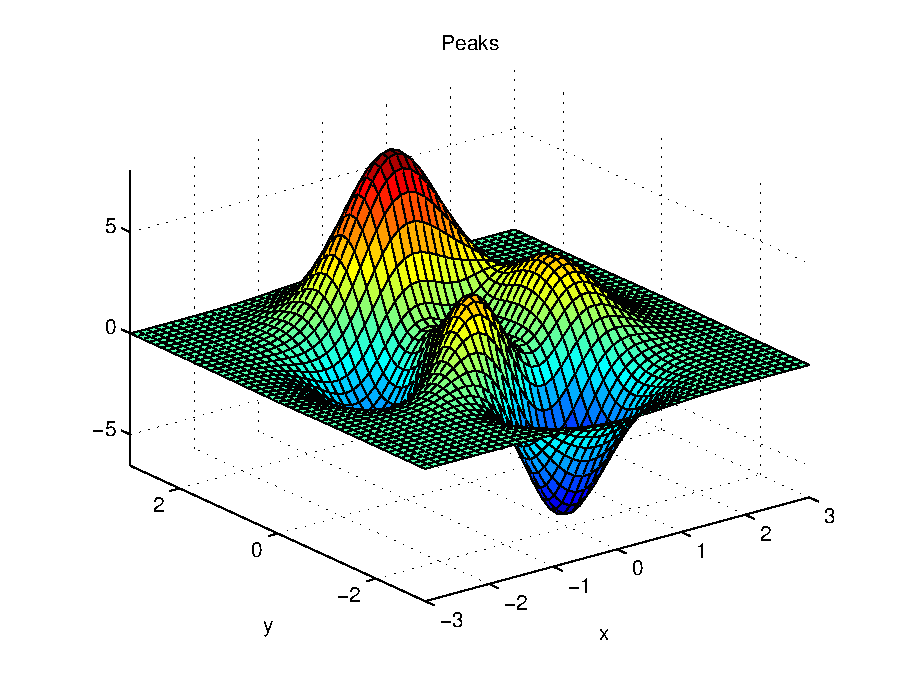
\includegraphics[width=12cm]{mcmthesis-aaa.eps}
% \caption{aa} \label{fig:aa}
% \end{figure}

% \lipsum[8] %\eqref{aa}
% \begin{equation}
% a^2 \label{aa}
% \end{equation}

% \begin{equation}
% e^{i \theta} = \cos \theta + i \sin \theta \label{bb}
% \end{equation}

% \[
%   \begin{pmatrix}{*{20}c}
%   {a_{11} } & {a_{12} } & {a_{13} }  \\
%   {a_{21} } & {a_{22} } & {a_{23} }  \\
%   {a_{31} } & {a_{32} } & {a_{33} }  \\
%   \end{pmatrix}
%   = \frac{{Opposite}}{{Hypotenuse}}\cos ^{ - 1} \theta \arcsin \theta \eqno(3)
% \]

% \lipsum[9]

% \[
%   p_{j}=\begin{cases} 
%   0,&\text{if $j$ is odd}\\
%   r!\,(-1)^{j/2},&\text{if $j$ is even}
%   \end{cases}
% \]

% \lipsum[10]

% \[
%   \arcsin \theta  =
%   \mathop{{\int\!\!\!\!\!\int\!\!\!\!\!\int}\mkern-31.2mu
%   \bigodot}\limits_\varphi
%   {\mathop {\lim }\limits_{x \to \infty } \frac{{n!}}{{r!\left( {n - r}
%   \right)!}}} \eqno (1)
% \]

\section{Analysis of the Problem}
  \indent \indent We consider the distribution of languages as the output of a function related to multiple factors, such as GDP, immigrants, population, imports, exports, and etc. These factors not only affect a country's language distribution, but also have an effect on other countries' languages. \\
  \indent So we build the model like this, assume ...

\section{Models and Methodology}
  \subsection{Time Series Prediction}
  \indent \indent In order to have an intuition about how the factors that have influence on languages will change in the next 50 years, we use the well-known ARIMA model to predict them. ARIMA model, i.e autoregressive integrated moving average model, is a widely used method for predicting time series. Considering these factors change over the time, and in order to simplify this problem, we regard them as factors only related to time. The ARIMA model can be represented as following form.

  \begin{equation}
    \left(1-\sum^p_{i=1}\sigma_i L^i\right)(1-L)^d X_t = \left(1+\sum^q_{i=1}\theta_i L^i\right)\epsilon_t
  \end{equation}

  \indent In the equation above, $L$ stands for Lag Operator, d$\in$Z, d$>$0.

  \indent Considering these factors we use vary randomly and are related to many other factors, so they are not stationary variables and can not be directly used int ARIMA model. So we calculate the difference of factors we study and apply ARIMA model on them. After getting the forecast result we calculate the accumulation to restore prediction result. Take the GDP prediction for an example, we collect the GDP of countries from 2002 to 2016, calculate the difference of adjacent years and use the $ARIMA$ model of $Python$ language. After this ARIMA model gives us the prediction of how the difference of a country's GDP will change in the next 50 years, we calculate the accumulation of this prediction values and regard the final sum as our prediction on this country's GDP.
  \indent The results we got from time series prediction show us the approximate trends about how these factors will change during the next 50 years. But limited by the amount of data we collected, it's not reasonable to predict a long term process with only a few data points. So we finally used the following PEIL model for a better prediction.

  \subsection{K-Means}

  \subsubsection{New Offices}

  \indent \indent In order to get the best locations for this company's six new offices, we resort to the power of social network. Concretely, we use data sampled in Twitter for 24 hours, which we think can represent the one day's social life of people around the world well. The data sampled from Twitter API gives us the information about the locations of uploaders, the language of tweets and the origin language of uploaders when he or she registered Twitter. 

  \indent Considering this company is a multinational service company and needs to be more multinational, the new offices of it should be close to its clients and information, which indicates places with many people around might be a good choice for these offices. So we mark the locations of tweets uploaders on a world map and use K-means algorithm to find centroids of different clusters of uploaders. Obviously, these centroids are centers of crowd and offer great opportunities for companies.
  
  \indent Because of the need for multi-language speakers of this company, it is important to consider the language environment of these new offices. To simplify this problem, we regard the uploaders whose tweets use different language from his or her registration language as a potential polyglot, so the language environment around them might be more open and attactive. Based on this assumption we pick those "polyglots" from our data and apply K-means algorithm on them. After setting $K$ to be equal to 8 (This company alreadly has two offices on Shanghai and New York, so the total offices it has will be 8), we got the following results.

  \begin{figure}[h]
    \small
    \centering
    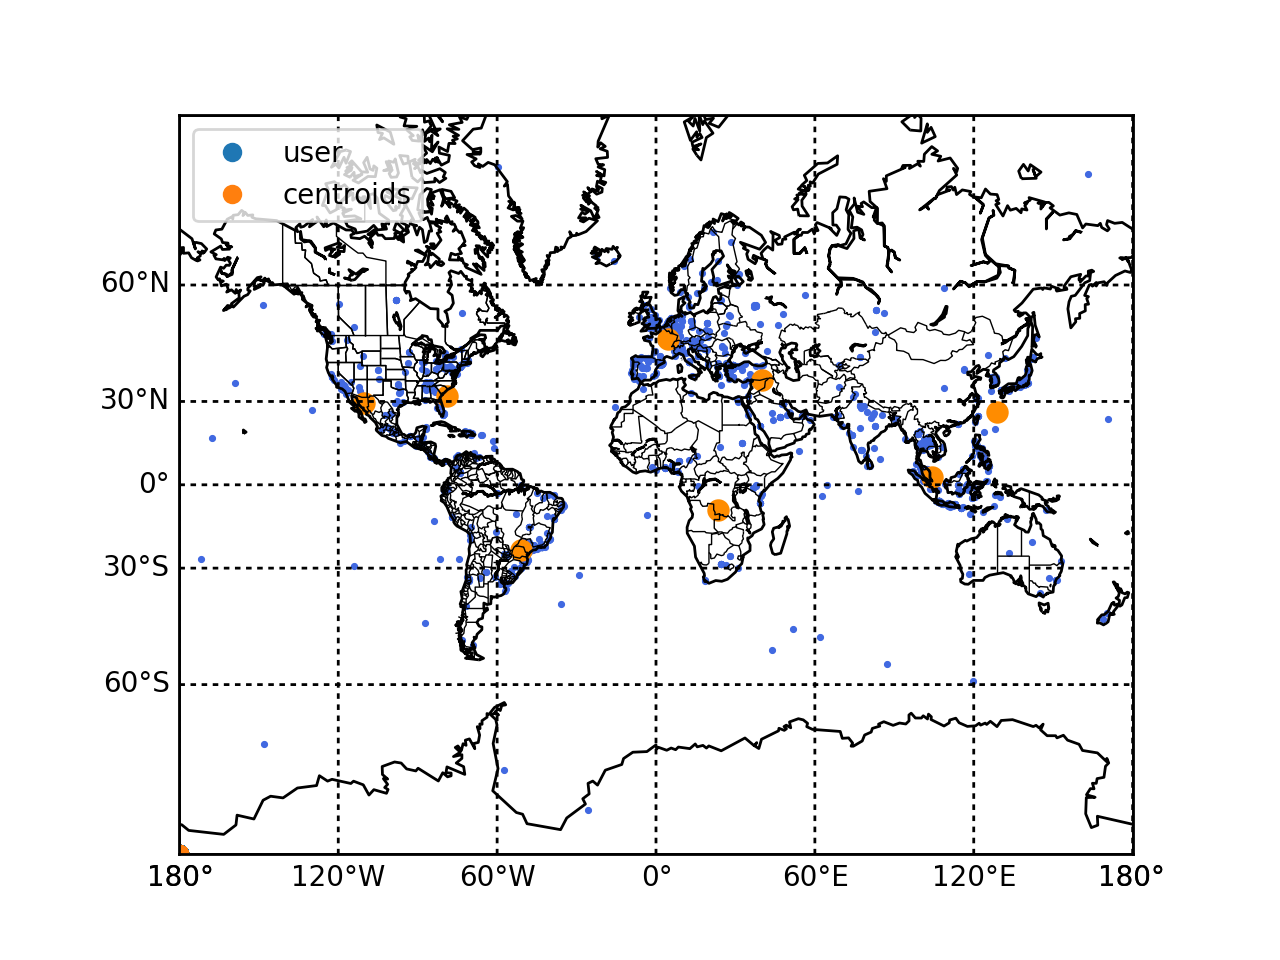
\includegraphics[width=12cm]{world_offices.png}
  \end{figure}

  \indent Our result shows all eight locations that is appropriate to set up new offices. Apart from the two offices that alreadly exist in Shanghai and New York (which may not be exactly on its true place on this map, but in consideration of sampling errors, we think it is still reasonable to regard the points lies on east coast of North America and China to be New York and Shanghai), we can still see the other six new offices. They are located in San Francisco, São Paulo, Paris, Jerusalem, Kinshasa and Singapore. It is shown that they are nearly located in seperated continents on earth, which is in accordence with the need to get a more open language environment.

  \indent In terms of what languages will be spoken in these six new offices, we still use the data from Twitter to help us decide. We collect tweets uploaders near the six new offices and count the types of languages of these tweets. Let us use the office in Paris as an example, we calculate what types of languages are used by uploaders around Paris and how many tweets are uploaded using corresponding language. The result can be shown as follows.

  \begin{figure}[h]
    \small
    \centering
    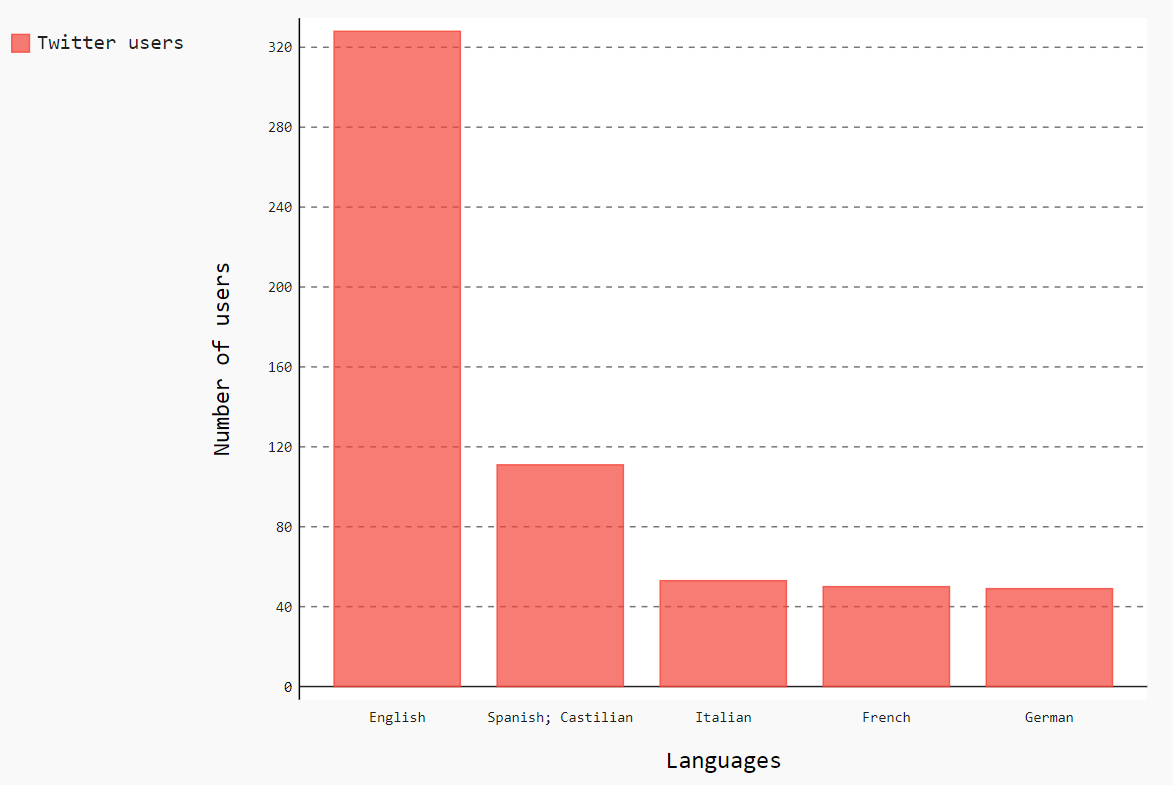
\includegraphics[width=10cm]{paris.png}
  \end{figure}

  \indent So languages spoken in the office in Paris might be English, Spanish, Italian, French and German. And here are the languages spoken in other new offices.
  \begin{itemize}
    \item Office in San Francisco: English, Spanish, French, Japanese and Portuguese.
    \item Office in São Paulo: Portuguese, Spanish, English, Japanese and Finnish.
    \item Office in Jerusalem: Turkish, English, Russian, Arabic and Japanese.
    \item Office in Kinshasa: English, Spanish, French, Portuguese and Afrikaans.
    \item Office in Singapore: Chinese Mandarin, English, Indonesian, Thai and Spanish.
  \end{itemize} 

  \indent The K-means model we use is from $Python$. It uses an effective k-means++ algorithm to speed up the total clustering process. The intuition of k-means++ algorithm can be interpreted as follows: when choosing the next centroid, always choose the centroid that is far from all centroids that have already been chosen. This meets with the desire to be more international because it disperses the new offices and make them distributed globally. 

  \subsubsection{Less Offices}

  \indent \indent The K-means model can also help us identify the best number of new offices. We transform the problem into finding best number of clusters in a data set. Here we use the elbow method, which is a convenient but also efficient way to find the best K in K-means algorithm. The key index of this method is SSE(sum of squared errors), which is defined as follows:
  \begin{equation}
    \mathop{SSE} = \sum^k_{i=1}\sum_{p\in C_i}\left|p-m_i\right|^2
  \end{equation}
  \indent Where $k$ stands for the number of clusters and $m_i$ denotes the centroid of cluster $i$, so $p$ is the point in cluster $i$. The elbow method tells us that generally when the number of clusters increases, the SSE of whole model will descend rapidly at first but slow down soon afterwards. So an "elbow" point will appear and it corresponds to the best number of clusters that the K-means algorithm should choose. Here is the elbow method result for this problem.

  \begin{figure}[h]
    \small
    \centering
    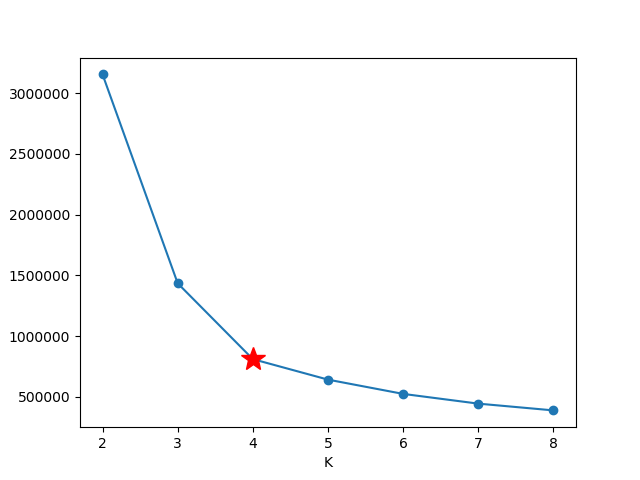
\includegraphics[width=12cm]{elbow_method.png}
  \end{figure}

  \indent According to this result, this company should open two more international offices, as the best number of clusters should be four. And after using the K-means algorithm above we got the result that the two new international offices should be located in Paris and São Paulo.
  
\section{Validating the Model}

\section{Conclusions}

\subsection{Conclusions for new offices}
\indent \indent We recommand the six new offices of this company to be located in are San Francisco, São Paulo, Paris, Jerusalem, Kinshasa and Singapore. Based on our assumptions above, these cities are centroids of open and vigorous environment, which means they are great places for this company to develop business. And with the languages each office might speak listed above, we can summarize that English, Chinese Mandarin, Spanish, French, Turkish and Portuguese might be the most common languages of these offices.

\indent Besides, using the elbow method above, we found that it might be better for this company to open just two new offices because this plan saves more resources and covers considerable amount of clients of the world. And using the K-means algorithm again we found that the two new offices should be located in Paris and São Paulo. 

\section{A Summary}

\section{Strengths and weaknesses}

\subsection{Strengths}
\begin{itemize}
\item 
\end{itemize}
\subsection{Weaknesses}
\begin{itemize}
  \item \textbf{Long-term predictions by K-means can't be made }\\
  The data we collected from Twitter is only one day's data. So we can use it to make short-term predictions. But the long-term prediction with K-means algorithm lacks the necessary data so its result in long term is not convincing.
\end{itemize}


\begin{thebibliography}{99}
\bibitem{1} D.~E. KNUTH   The \TeX{}book  the American
Mathematical Society and Addison-Wesley
Publishing Company , 1984-1986.
\bibitem{2}Lamport, Leslie,  \LaTeX{}: `` A Document Preparation System '',
Addison-Wesley Publishing Company, 1986.
% \bibitem{3}\url{http://www.latexstudio.net/}
\end{thebibliography}

\begin{appendices}

\section{First appendix}

\indent \indent Here are simulation programmes we used in our model as follow.\\

% \textbf{\textcolor[rgb]{0.98,0.00,0.00}{Input matlab source:}}
% \lstinputlisting[language=Matlab]{./code/mcmthesis-matlab1.m}

\section{Second appendix}

% some more text \textcolor[rgb]{0.98,0.00,0.00}{\textbf{Input C++ source:}}
% \lstinputlisting[language=C++]{./code/mcmthesis-sudoku.cpp}

\end{appendices}
\end{document}